\chapter{Server-Side Implementation}
\lhead{\emph{Server-Side Implementation}}
\label{chapter:server}

The purpose of the server is to receive image data from the rover, produce a 3D environment from this data, and feed back control inputs from the user. This is all done within the framework of the 3D game engine Unreal Engine 4 \cite{unreal}. Unreal 4 was chosen because it provides easy interfacing with almost any VR headset on the market without large rewrites of the code, it is simple to integrate with OpenCV, and is free to use. The structure of any Unreal program is very complicated, as the engine does a lot in the background across many threads. The implementation of this project within the Unreal environment (Figure \ref{fig:unreal}) consists of a receive thread that receives and processes the images and updates the 3D model, and a part of the game thread (the Unreal thread that handles game logic) that handles and sends user input 20 times a second. The fact that the 3D model is updated on a thread separate to the rendering of the images that are sent to the headset is what allows the headset to run at an unrelated and significantly faster frame rate than the model is being updated at.

\begin{figure}[H]
    \begin{center}
      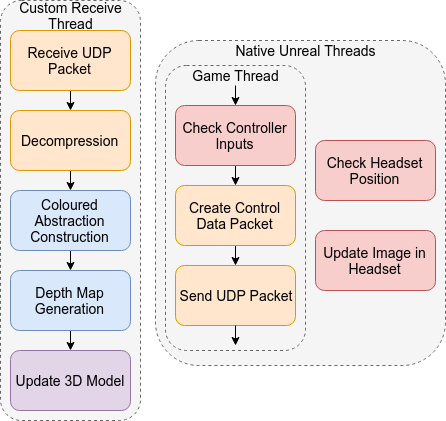
\includegraphics[width=0.75\textwidth]{Figures/Unreal.png}
      \caption[Server Program Structure]{Server Program Structure. Red blocks are standard Unreal functionality, yellow blocks are communications related, blue blocks are OpenCV based, and the purple block is custom integration with the Unreal environment. The blocks within the game thread run 20 times a second. When these blocks are not running, the game thread is handling other game logic within the environment.}
      \label{fig:unreal}
    \end{center}
\end{figure}

\section{Depth Map and Abstraction Construction}

For a depth mapping algorithm to function accurately, the 2 images it receives must be rectified (established in Section \ref{subsection:depth}). The rectification parameters for the cameras in our system have been calculated using a set of programs provided by Sourish Ghost \cite{calibgit}. The rectification is then applied using these parameters just before the depth maps are calculated (Figure \textcolor{red}{[RECTIFICATION PICS]}).

When selecting a depth mapping algorithm, the major factors to consider were speed and performance with abstracted images. The use of abstractions makes demonstrations of the algorithms with full images of little help; there is no guarantee that the algorithms would be able to map depth for edge detected lines as well as if they were full images, if at all, since this is not what they are designed for. Three different depth mapping algorithms were tested: StereoBM, StereoSGBM, and Libelas. StereoBM and StereoSGBM are a block matching and semi block matching algorithm provided by OpenCV \cite{OpenCV}, and Libelas is a more complex algorithm provided by the Autonomous Vision Group \cite{geiger2010efficient}. Of the three algorithms presented, StereoBM is the fastest and Libelas the slowest (Figure \textcolor{red}{[SPEED GRAPH]}). 

When tested on images received from the rover, StereoBM produced reasonable results (Figure \textcolor{red}{[DEPTH COMPARISON]}), producing approximations of depth along the edges in the image and producing noise otherwise. The noise is unsurprising and unconcerning, as the algorithm is attempting to find depth within the areas of the image that are simply black space, and will be discarded anyway. StereoSGBM is a slower algorithm then StereoBM, however it produces similar results, leading to it being quickly discarded as an option. Libelas, a significantly more complicated option, does not produce any reasonable results with edge detected images. The intelligence of Libelas may have led to it attempting to find indicators within the images that no longer exist after they have been edge detected. Whatever the case may be, the logical choice from this set of options is StereoBM.

To produce a 3D model from one of the depth maps produced by StereoBM, the depth calculated on the edges of objects must be applied to the spaces between them. The method chosen for this task was to apply Weighted Least Squares filtering to the depth map (Figure \textcolor{red}{[FILTERING]}). This is effective in filling most spaces in the map with depth found in the edges adjacent to them. Unfortunately, regardless of the angle to the camera that an object sits at, the filtering will give it flat depth. This results in surfaces like the floor or the ceiling being inaccurately represented, however it does not significantly affect most objects.

While the individual depth maps (post filtering) are reasonable approximations of the space being viewed, the depth of a single object with be inconsistent between frames, due to inconsistencies between edge detected frames. When viewed as a video feed, most objects will oscillate slightly, with greater oscillations in objects that are more ambiguous or less consistent in the edge detected frames. This issue is mitigated in the system by taking a running average, the weighting of the frames in the average reducing with the age of the frame. This increases consistency substantially at the expense of a minor reduction in responsiveness.

The construction of the coloured abstraction is as addressed in Chapter \ref{chapter:abstract}. The seed point/average colour pairs are each used to flood fill "Edge Detected Img 1" from Figure \ref{fig:system}, producing the full abstraction that is to be applied as a texture to the 3D model generated from the depth map.

\section{3D Model Generation}

To generate a 3D model dynamically based on image data, an Unreal Engine 4 class that allows for mesh generation at run-time is required. Although more intelligent options are available as add-ons, the core Unreal 4 class "procedural mesh" was selected due to its simplicity and compatibility with OpenCV. The class is used as a basis for the generation of a grid based mesh (Figure \ref{fig:mesh}).

\begin{figure}[H]
    \begin{center}
      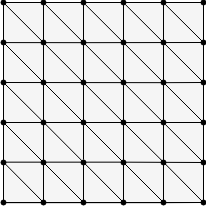
\includegraphics[width=0.6\textwidth]{Figures/mesh.png}
      \caption[Mesh Grid Segment]{Mesh Grid Segment.}
      \label{fig:mesh}
    \end{center}
\end{figure}

Each pixel in the depth map is mapped to a vertex in the mesh, resulting in a grid of 320x240 vertices for 320x240 pixel images. The colour value of each depth map pixel is mapped to the Z component of its corresponding vertex, leading to the bright pixels in the depth map (close objects) generating vertices that are pushed forward from the grid. When this grid is placed an appropriately realistic distance from the the user in the headset, the close objects in the depth map will be pushed closer to the user. When the full coloured abstraction is then applied to the mesh as a texture, the pixels once again mapping 1:1 to the vertices, the space the rover is observing is finally being portrayed in VR (Figure \textcolor{red}{[WITHOUT THEN WITH TEXTURE]}).